%-------------------------------------------------------------------------------
\section{Design}
%-------------------------------------------------------------------------------
\iffalse
\begin{figure}[t!]
    \centering
    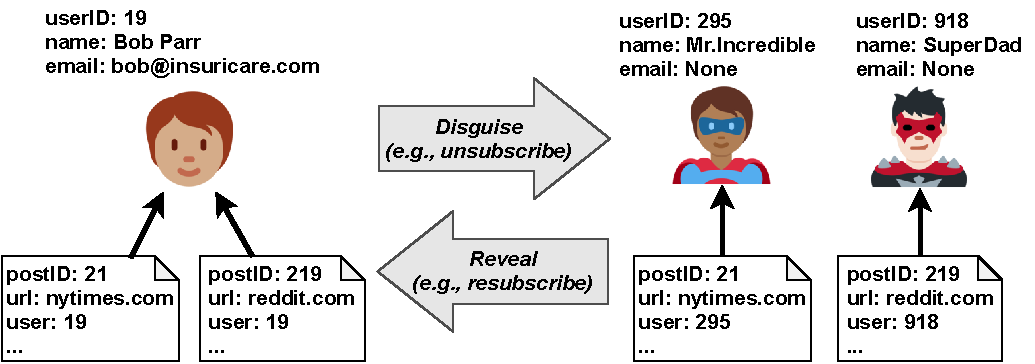
\includegraphics[width=0.5\textwidth]{img/disguises}

    \caption{Disguises move the target object (in this example, a user Bob) from an identity-revealing
    guise to privacy-preserving guises.}
    \label{fig:example}
\end{figure}
\fi

\begin{figure*}[t!]
    \centering
    \footnotesize
\begin{tabular}{@{}c|c|c|c@{}}
\textbf{User Transformation Spec} & \textbf{User Object} & \textbf{Guise 1} &
    \textbf{Guise 2} \\
\begin{lstlisting}[language=Rust]
"id":       IDAttribute,
"name":     Gen(Random),
"active":   Gen(Default(false)),
"darkmode": CopyAll,
"notifs":   CopyOnce+Gen(Default(false)),
"tag_id":   GenForeignKey,
\end{lstlisting}
    &
\begin{lstlisting}[language=Rust]
"id":       19,
"name":     BobParr,
"active":   true,
"darkmode": false,
"notifs":   true,
"tag_id":   11
\end{lstlisting}
&
\begin{lstlisting}[language=Rust]
"id":       295,
"name":     MrIncredible,
"active":   false,
"darkmode": false,
"notifs":   true,
"tag_id":   81483
\end{lstlisting}
&
\begin{lstlisting}[language=Rust]
"id":       918,
"name":     SuperDad,
"active":   false,
"darkmode": false,
"notifs":   false,
"tag_id":   15592
\end{lstlisting}
\end{tabular}
    \caption{Creating two guises of an example user (of a synthetic application schema).}
    \label{fig:guises}
\end{figure*}



\sys's design centers around the key observation that user data may expose identifying information
both directly from its contents, and indirectly through its structural correlations to other
application data. 

In order to capture exactly which data contents, and which data correlations may be
identity-sensitive, \sys models an application's data as a graph of \emph{entity} nodes and edges.
Each entity type corresponds to an application datatable, such as a stories, users, or votes table.
Entities are linked in the entity graph by foreign key relationships: table columns that act as
foreign keys to other tables create child-parent relationships between entities, where the child
entity holds the parent entity's identifier as a foreign key. \sys also includes
abstract entities in the graph, where the keys may be non-referential identifiers that refer to
abstract, non-table entities (e.g.,\ a \texttt{thread\_id} column in the comments table).  Edges in
the graph---foreign or abstract key relationships---represent correlations between the nodes of the
graph, namely individual entities.

Unsubscription policies center around the abstraction of \emph{ghost entities}. A ghost entity is
more than an anonymized version of a real entity: a real entity may be replaced by multiple ghost
entities, breaking up correlations associated with the real entity; and ghost entities can be
partially randomized, partially custom generated, and partially clones of the real entities. 
%achieving fine-grained data retention and anonymization. 
Pre- and post-unsubscription state differ by the presence of ghost entity nodes and edges, which
have taken the place of real entities and edges.

While \sys operates on a specific instance of the application entity graph, the developer reasons
only about the \emph{types} of individual entities and the \emph{types} of entity edges that may be
instantiated in the graph. This allows unsubscription policies to be specified statically using only
the application schema, while \sys ensures that any instance of the application entity graph
satisfies the state specified in the policy.

To exemplify \sys's policy choices, we demonstrate how each choice changes the state of user, story,
and vote entities in a simplified variant of the Lobster's schema, shown in Figure~\ref{fig:schema}.

\subsection{Ghosting Entity Attributes}
\label{sec:ghosting}
Developers must first define how ghost entities are generated from a real entity.
\sys assumes entities have three kinds of attributes: a unique identifier attribute; 
value (non-referential) attributes such as timestamps or usernames; and 
edge (referential foreign key) attributes that identify correlations to parent entities. 
Value attributes may directly expose identifying information from its
contents, and edge attributes represent potentially sensitive structural correlations. 
Developers specify how \sys should generate each of these attributes in a ghost entity.

\sys generates ghost entities for two reasons: to replace correlations to real parent entities,
or to add new correlations from ghost children to real parents.

\sys always generates ghost entities with unique identifier attribute values.

For each value attribute of each entity type, developers specify a \emph{value ghosting policy}.
Value ghosting policies take as input a current entity's attribute value, and return a ghosted
version. Developers can specify whether the ghosted replacement should be random, a default value,
or generated from the original value via a custom function provided by the developer.
Figure~\ref{fig:example} demonstrates examples of these various policies on a range of
value attributes.

For each edge attribute, or foreign key relationship, of the entity type, the developer specifies an
\emph{edge ghosting policy} that specifies how and when the edge can be decorrelated and ghost
entities created.  The following section describes edge ghosting policies in more detail.

Figure~\ref{fig:policy} shows pseudocode for \sys's policy specification types.
%Using ghost generation policies, \sys creates ghost entities to replace unsubscribed entities. 

%During unsubscription, \sys traverses the current instance of the application entity graph with the
%top-level unsubscribing user node as the root in order to find all possible graph edges and nodes
%that may be sensitive. \sys then applies the applies the appropriate decorrelation policy to all
%sensitive edges depending on the edge type, generating ghost nodes with ghosted attributes to
%replace real nodes as specified.
%
%After ghosts are generated from the template entity, \sys returns a copy of the template entity to
%the unsubscribing user, which if returned upon resubscription, allows \sys to restore the original
%value. If the user does not wish to store this data, resubscription retains the ghosted value in
%%place of the original.
%Resubscription requires the user to return the original
%data to restore the original value.

\lyt{TODO ghost generation should be separated into two parts: generating ghost parents, and
generating ghost children. The whole CLONE/GENERATE/CLONE-ONE menu should be per ghost entity type,
rather than per edge ghosting policy, and apply to both value and edge attributes.}

\subsection{Edge Ghosting Policies}
Developers specify edge ghosting policies on a particular edge type, identified by a pair of parent
entity type and child entity type. The edge ghosting policy is associated with an edge attribute,
namely a foreign key column, of the child entity. Figure~\ref{fig:example} shows three different
child-parent edge types: stories-users, votes-users, and votes-stories.

For each edge type, developers choose between options that (1) decorrelate the edge, replacing
the existing one with one to a ghost parent; (2) retain the edge but ghost the value attributes of the
parent node; (3) remove the edge entirely; or (4) add false edges to introduce noise.
The following sections explain each policy in more detail, followed by a description of how \sys
generates ghost edges for these policies.


\lyt{TODO Figure~\ref{fig:edge_policies} depicts how the state of stories-users edge types changes depending
on the policy.}

\paragraph{Policy 1: Decorrelate.}
\sys decorrelates edges of this type by breaking the link from child entity to parent entity.
Correlations to parents are replaced by correlations to a unique ghost parent, generated using the
real parent as a template.  \sys links each child to a unique ghost by replacing each child's edge
attribute (foreign key column) with a unique ghost parent's identifier. 
All real parents are removed, and their data returned to the unsubscribing user.

\paragraph{Policy 2: Retain.}
Application developers specify that these types of edges cannot be decorrelated: children 
that are correlated with the same, single parent should remain correlated with the same 
parent. Developers should select this option only if the developer knows that these correlations
cannot collectively leak identifying information, and/or if the application's functionality would be
impacted by deleting or decorrelating this type of edge.

For each parent, \sys generates a single ghost parent entity using the parent as a template, and
links all children to this ghost by replacing the childrens' edge attribute with the ghost's
identifier.

\paragraph{Policy 3: Delete.}
\sys deletes the edge by removing the child entity and any descendants.  Developers should select
this edge policy option only if this type of edge cannot be decorrelated while retaining application
semantics, but retaining edges to a shared parent would reveal too much identifying information.
All removed entity data is returned to the unsubscribing user.

\paragraph{Policy 4: Desensitize.}
Finally, the developer has the option to \emph{desensitize} correlations. This edge policy option
allows edges that cannot be decorrelated to be conditionally retained or removed.

The developer specifies a \emph{sensitivity threshold $\sigma$} greater than 0 and less than 1.  A
sensitivity threshold for an edge specifies the maximum proportion of edge instances of a certain
type that may connect to \emph{sensitive} entities (i.e.,\ entities transitively correlated to the
initial entity being unsubscribed). 

At a high level, the sensitivity threshold for a particular edge type estimates how much identifying
information may leak from edge instances of that type.  For any given edge type, developers can
determine an appropriate sensitivity threshold by approximating how much identifying information may
be leaked if edges of this type with the same parent key \emph{all} correlate (even indirectly) back
to the entity being unsubscribed. In other words, what happens if all children of edges of this type
(with the same parent) are sensitive?

For example, consider the edge from stories to tags. If all the stories tagged with the same parent
tag in the entity graph were written by some (unsubscribed) user, would the story-tag correlation be
problematic? The answer may be yes: perhaps tags are customizable by the user, and any story with
that tag will clearly belong to the unsubscribed user. In other cases, the answer may be no: even
though the tag is only correlated with sensitive stories, the tag indicates nothing about who may
have authored the stories.

For many cases, the answer may lie somewhere in the middle: it is problematic if \emph{all} of
children of edge of this type are sensitive, but perhaps it is acceptable if only a fraction of
children of this edge type are sensitive. The maximum value for this fraction is the sensitivity
threshold.  For example, a reasonable sensitivity threshold might be $\sigma = 0.1$ for stories-tag
key relationships: less than 10\% of all stories with a specific tag key should have been correlated
(even indirectly) with an (unsubscribed) user. 

The developer chooses between two desensitization options:
\begin{enumerate} 
    \item \textbf{Add ghost correlations}: For each parent of this edge type, \sys
            generates ghost children entities using the appropriate value ghosting policies and an
            existing child entity as a template. All ghost children point to the parent (share the
            same edge attribute value).  \sys generates enough ghost children that the sensitivity
            threshold is met.  Note that if the generated ghosts are easily distinguished from
            actual entities, there is little privacy benefit from generating ghost entities to meet
            the threshold.

\item \textbf{Remove sensitive correlations}: \sys removes sensitive children and their dependencies
    until the threshold is met. (Note that if there are no unsensitive children, all sensitive
    children must be removed). All removed entity data is returned to the unsubscribing user.
\end{enumerate}

\paragraph{Creating Ghost Edges.}
Several of the edge ghosting policies choices requires \sys to generate one or many ghost entities
to create ghost edges. These ghost parents or children replace real edges or add ghost edges to the
entity graph.  Depending on the policy, \sys uses either a real parent or a real child of the
edge as a template. 

While developers specify ghost generation policies as described in Section~\ref{sec:ghosting}, \sys
cannot simply apply the specified ghosting policies for value attributes.  This is because the
application may require that only \emph{some} of the generated ghosts contain ghosted values. In
particular, perhaps the application requires that one or all of the ghosts clone the original value
of the template entity. For example, an application's policy may generate several ghost votes to
create ghost edges to a parent story. However, the application may want to clone the original vote
value in exactly \emph{one} ghost vote, and generate ghosted vote values for all other ghost votes,
so that the total vote count remains unchanged. 

For each edge ghosting policy, \sys requires the developer to specify whether value attributes
should be cloned or ghosted, choosing between the following options:
\begin{itemize}
    \item \textbf{Clone-All:} All ghosts generated from the same template will share the same value
        for this column attribute as the template.

    \item \textbf{Generate-All:} \sys uses the appropriate value ghosting policy for this
        value attribute to generate a value for each ghost, using the template entity's value
        as input.

    \item \textbf{Clone-One:} One ghost entity shares the same value for the column attribute as the
        template; \sys uses the appropriate value ghosting policy to generate the attribute value
        for all other ghosts generated from this template.
\end{itemize}

\sys generates a unique identifier attribute for each ghost.  To generate edge attributes, \sys
initially clones the edge (foreign key) value of the template entity for all ghost entities.  \sys
then looks up the appropriate edge ghosting policy for that edge type, and applies it to all the
generated ghosts. For example, if the entity has a decorrelatable edge to a parent entity, then \sys
recursively generates and links all ghost entities to unique ghost parent entities. \sys does not
recursively apply edge ghosting policies if the edge policy specifies that the generated ghosts
should be linked to a particular parent, as in the \texttt{Desensitize} policy. 

\subsection{Resubscription}
Several policies (\texttt{Decorrelate/Remove/Desensitize\-Remove}) return the decorrelated or deleted
entity data to the unsubscribing user. \sys additionally returns the identifier attributes of all
generated ghosts, and, for each decorrelated entity, the set of ghosts that replaced that entity's
correlations.

Upon resubscription, the user returns this ghost metadata and any removed entity data, allowing \sys
to remove any created ghost entities, recorrelate entities back with the correct real entity, and
restore removed entities and their descendants. \sys allows the application developer or user to
ignore any entity data returned by \sys upon unsubscription, but consequently cannot restore this
data when the user resubscribes.  This choice reduces the amount of user-side storage required for
resubscription when the data can be easily re-initialized, is simply too large to store, or plays no
essential role in using the application.
        
\subsection{\sys's Execution Algorithm}

\lyt{NOTE---EVERYTHING PAST HERE IS OLD. (Need to modify to fit the rewritten above design.)}

Given this specification and an entity to be decorrelated as input, \sys acts as follows:
\begin{enumerate}
    \item \textbf{Parent-Child Traversal:} \sys traverses the entity graph starting from the input entity,
        going down parent to child edges (and halting if it detects a cycle).  As it traverses,
        \sys collects the edges it has traversed. 
    
    \item \textbf{Parent-Child Decorrelation:} Post-traversal, \sys acts on each edge instance
        according to the specified decorrelation relationship policy for that edge's type: if no
        policy is specified, \sys does nothing. If edges can be decorrelated, \sys generates
        ghost parent entities and new edges between child and ghost parent entities using the
        appropriate ghost entity generation policy. If edges cannot be decorrelated and should be
        retained or deleted, \sys does nothing or removes the child and edge respectively. 
    
        If there is a sensitivity threshold for the edge's type, \sys ensures the
        sensitivity of the edge is below $t$'s threshold, providing the edge type and the edge's
        parent key to the procedure described in Section~\ref{sensitivity_algo}. 

    \item \textbf{Child-Parent Decorrelation:} Next, \sys takes the children of all traversed edge
        instances, and considers the set of edges from these children to other parents
        \emph{not} traversed by \sys during the decorrelation phase. (In other words, these
        children entities have multiple key relationships to several parent entities, one of
        which is connected via a chain of parent-child edges to the input entity).

        Intuitively, children of edges traversed by \sys share a connection with the initial
        entity being decorrelated. Edges \emph{from} these children to other parent entities may
        thus leak sensitive identifying information. 

        \sys acts on these edges according to the specified decorrelation relationship policy for
        each edge's type. If these edges can be decorrelated, \sys generates ghost parent entities
        for each sensitive child.  If these edges cannot be decorrelated and should be retained or
        deleted, \sys does nothing or removes the child and edge respectively. 
        
        Otherwise, if there is a sensitivity threshold for the edge type, then \sys limits the
        proportion of edges of that type that connect to sensitive entities (the children of
        traversed edge instances) to below the threshold. 
        For each edge with type $t$ in this set of edges, \sys ensures the
        sensitivity of the edge is below $t$'s sensitivity threshold, providing the edge type and the edge's
        parent key to the procedure described in Section~\ref{sensitivity_algo}. 

        \sys optionally allows developers to specify that edges have \emph{weaker}
        decorrelation policies in the child-to-parent direction than from parent-to-child: this
        allows expression of policies where it is safe to retain links if \emph{only the child} is
        sensitive, but where the link should be decorrelated, removed, or desensitized if
        \emph{both} the child
        and parent are sensitive. For example, perhaps a user wants to ensure that their link to
        sent messages are decorrelated, but links from the message to the recipient users 
        can still be retained.
\end{enumerate}

An example of these three decorrelation steps is shown in Figure~\ref{fig:algo}.

\subsubsection{Achieving the Sensitivity Threshold}
\label{sensitivity_algo}
Let $E$ be the subset of edges traversed by \sys in Step 1 of execution. 
Given an edge type $t$ with sensitivity threshold $\sigma_t$, and a parent key $k$ of an instance of
edge type $t$, 
    \begin{itemize}
        \item \sys computes $N_{sensitive}$, the number of edges of type $t$ with parent $k$ in the entity graph that share 
            a child node with edges in $E$.
        \item \sys computes $N_{all}$, the total number of edges of type $t$ with parent $k$
            in the entity graph of edge.
        \item \sys computes $N_{sensitive}/N_{all}$, the \emph{sensitivity} of edges of type $t$
            with parent $k$.
        \item If the sensitivity exceeds $\sigma_t$ and the child entity type has an associated ghost entity policy, \sys
            generates ghost children and edges of type $t$ from these children to parent
            key $k$. This lowers the sensitivity by increasing $N_{all}$. Note that this may also
            create other ghost parents for the generated ghost children if these children have more
            than one column representing a foreign key relationship.
        \item Otherwise, if the sensitivity exceeds $\sigma_t$ but ghosts cannot be generated,
            \sys removes the children of edges in $E_t$ with parent $k$, thus lowering the
            sensitivity by lowering $N_{sensitive}$.
    \end{itemize}

Note that the initial sensitivity for an edge of type $t$ with parent $k$ from Step 2 (parent-child
decorrelation) is always 1. Because \sys traverses from parent to child, if one edge of type $t$ with
parent $k$ were collected by \sys, then \emph{all} edges of type $t$ with parent $k$ were collected
by \sys. 

However, the initial sensitivity for an edge of type $t$ with parent $k$ from Step 3 (child-parent
decorrelation) may be very low: other parents of children touched by \sys may have many
non-sensitive children (e.g.,\ a tag may have many stories not authored by the user being
decorrelated).

\begin{figure}[t!]
    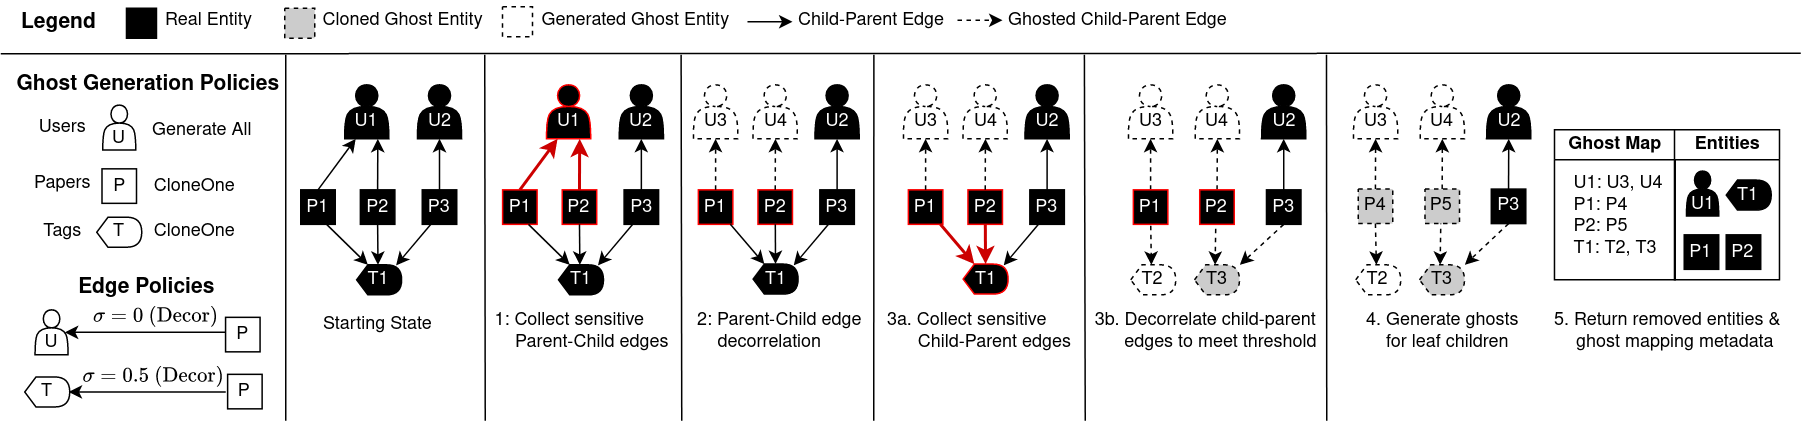
\includegraphics[width=.5\textwidth]{img/algo}
    \label{fig:algo}
    \caption{Examples of \sys's execution.}
\end{figure}

%\paragraph{Example policy.}
%We can imagine an application tin which only the sum of votes per story is ever queried by the application; clusters of
%votes around stories can therefore remain without leaking identifying information, and are thus
%assigned Policy 1, ``Do Not Decorrelate (Retain)''. 
%Decorrelation does propagate to the votes themselves, which are clustered by a \texttt{location} attribute; 
%this cluster by location can have a different decorrelation policy that generates ghost locations by
%randomizing the location, breaking up the cluster. 
%

%\sys provides a menu of unsubscription policy choices that allow developers to choose how to
%\emph{ghost} individual data record content, and how to \emph{decorrelate} sensitive correlations. 
%Specifying the policy requires nothing more than the application schema: ghosting policies act on
%application datatables and on foreign key relationships between tables.
%Table column values can be ghosted---removed, anonymized, or modified---in application-specific
%ways; and correlations can be broken, removed, or desensitized by adding noise. This gives
%developers the flexibility to specify fine-grained policies that properly de-identify a user, while
%retaining data as necessary for the application.

%\sys must pinpoint exactly which data and correlations may be
%identity-sensitive, and allow developers to specify exactly what the post-unsubscription state of
%this data should be.

